%##################################################
\frame{
\frametitle{Email- und Kalenderanbindung}
	\begin{block}{Kommunikation mit Hochschul-Content}
		\begin{itemize}
			\item Hochschul-interne Daten über Content System für \textbf{Kalender} und \textbf{Email}
			\item Content-Zugriff und \textbf{Update bei Internetzugriff} des Mobilfunktgeräts
		\end{itemize}
	 \begin{minipage}{0.6\linewidth}
  		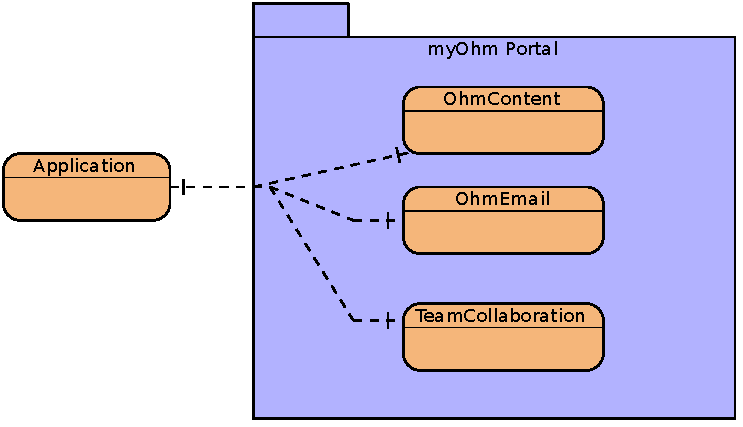
\includegraphics[width=0.9\textwidth]{../grafiken/OhmCollab.pdf}
    \end{minipage}
    \begin{minipage}{0.38\linewidth}
        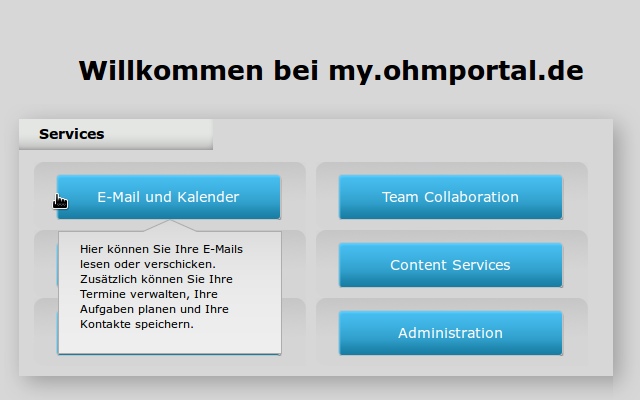
\includegraphics[width=1.0\textwidth]{../grafiken/myOhm.png}
    \end{minipage}
    	\end{block}
}

\frame{
\frametitle{Setup Skript}
	\begin{block}{Einrichten des Ohm Content}
	\begin{itemize}
		\item Standardapplikationen von Android für Email und Kalender werden genutzt
		\item \textbf{Installationsskript} soll das Einrichten aller Ohm Content Applicationen erleichtern
		\item Daten, die der Benutzer eingeben muss: 
		\begin{itemize}
			\item Benutzername
			\item Passwort
		\end{itemize}
		\item \textbf{Serveradresse und Port} sind hochschulabhängig und hinterlegt
	\end{itemize}
	\end{block}
}


%
%\frame{
%\frametitle{Datenhaltung}
%	\begin{block} {Content Management System (CMS)}
%	\begin{itemize}
%		\item CMS zum Verwalten von Inhalten
%		\item Verschiedene Benutzerrollen:	
%			\begin{itemize}
%				\item Administrator: Bearbeitung von Design und Inhalt
%				\item Redakteuer: Bearbeitung von Inhalt
%			\end{itemize}
%		\item $\rightarrow$ Hochschule benutzt bereits CMS-Systeme für Inhalte der Webseite. \\\textbf{Vorteil: zusätzliche Schulung nicht notwendig} 
%	\end{itemize}
%	\end{block}
%	\begin{block}{Diagramm}
%		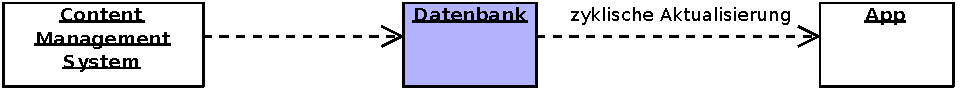
\includegraphics[width=1.0\textwidth]{../grafiken/DB.pdf}
%	\end{block}
%}


